\documentclass{article}
\usepackage{graphicx, tikz-cd, float, titlepic, booktabs} % Required for inserting images
\usepackage{pgfplots}
\pgfplotsset{compat=1.15}
\usepackage{mathrsfs}
\usetikzlibrary{arrows}
\usepackage{amsmath, amssymb, amsthm, amsfonts, siunitx, physics, gensymb}
\AtBeginDocument{\RenewCommandCopy\qty\SI}
\usepackage[version=4]{mhchem}
\usepackage[most,many,breakable]{tcolorbox}
\usepackage{xcolor, fancyhdr, varwidth}
\usepackage[Glenn]{fncychap}
%Options: Sonny, Lenny, Glenn, Conny, Rejne, Bjarne, Bjornstrup
\usepackage{hyperref, cleveref}
\usepackage{icomma, enumitem} %comma as decimal and continue enumerate with [resume]
\usepackage{plimsoll} %use standard state symbol with \stst
\usepackage[danish]{babel}
%%%%%%%%%%%%%%%%%%%%%%%%%%%%%%
% SELF MADE COLORS
%%%%%%%%%%%%%%%%%%%%%%%%%%%%%%
\definecolor{myg}{RGB}{56, 140, 70}
\definecolor{myb}{RGB}{45, 111, 177}
\definecolor{myr}{RGB}{199, 68, 64}
\definecolor{mytheorembg}{HTML}{F2F2F9}
\definecolor{mytheoremfr}{HTML}{00007B}
\definecolor{mylenmabg}{HTML}{FFFAF8}
\definecolor{mylenmafr}{HTML}{983b0f}
\definecolor{mypropbg}{HTML}{f2fbfc}
\definecolor{mypropfr}{HTML}{191971}
\definecolor{myexamplebg}{HTML}{F2FBF8}
\definecolor{myexamplefr}{HTML}{88D6D1}
\definecolor{myexampleti}{HTML}{2A7F7F}
\definecolor{mydefinitbg}{HTML}{E5E5FF}
\definecolor{mydefinitfr}{HTML}{3F3FA3}
\definecolor{notesgreen}{RGB}{0,162,0}
\definecolor{myp}{RGB}{197, 92, 212}
\definecolor{mygr}{HTML}{2C3338}
\definecolor{myred}{RGB}{127,0,0}
\definecolor{myyellow}{RGB}{169,121,69}
\definecolor{myexercisebg}{HTML}{F2FBF8}
\definecolor{myexercisefg}{HTML}{88D6D1}
%%%%%%%%%%%%%%%%%%%%%%%%%%%%%%%%%%%%%%%%%%%%%%%%%%%%%%%%%%%%%%%%%%%%%%
% Box environments for theorems and problems
%%%%%%%%%%%%%%%%%%%%%%%%%%%%%%%%%%%%%%%%%%%%%%%%%%%%%%%%%%%%%%%%%%%%%
\setlength{\parindent}{1cm}
%================================
% Question BOX
%================================
\makeatletter
\newtcbtheorem{question}{Opgave}{enhanced,
	breakable,
	colback=white,
	colframe=myb!80!black,
	attach boxed title to top left={yshift*=-\tcboxedtitleheight},
	fonttitle=\bfseries,
	title={#2},
	boxed title size=title,
	boxed title style={%
			sharp corners,
			rounded corners=northwest,
			colback=tcbcolframe,
			boxrule=0pt,
		},
	underlay boxed title={%
			\path[fill=tcbcolframe] (title.south west)--(title.south east)
			to[out=0, in=180] ([xshift=5mm]title.east)--
			(title.center-|frame.east)
			[rounded corners=\kvtcb@arc] |-
			(frame.north) -| cycle;
		},
	#1
}{def}
\makeatother
%================================
% DEFINITION BOX
%================================

\newtcbtheorem[]{Definition}{Definition}{enhanced,
	before skip=2mm,after skip=2mm, colback=red!5,colframe=red!80!black,boxrule=0.5mm,
	attach boxed title to top left={xshift=1cm,yshift*=1mm-\tcboxedtitleheight}, varwidth boxed title*=-3cm,
	boxed title style={frame code={
					\path[fill=tcbcolback]
					([yshift=-1mm,xshift=-1mm]frame.north west)
					arc[start angle=0,end angle=180,radius=1mm]
					([yshift=-1mm,xshift=1mm]frame.north east)
					arc[start angle=180,end angle=0,radius=1mm];
					\path[left color=tcbcolback!60!black,right color=tcbcolback!60!black,
						middle color=tcbcolback!80!black]
					([xshift=-2mm]frame.north west) -- ([xshift=2mm]frame.north east)
					[rounded corners=1mm]-- ([xshift=1mm,yshift=-1mm]frame.north east)
					-- (frame.south east) -- (frame.south west)
					-- ([xshift=-1mm,yshift=-1mm]frame.north west)
					[sharp corners]-- cycle;
				},interior engine=empty,
		},
	fonttitle=\bfseries,
	title={#2},#1}{def}
\newtcbtheorem[]{definition}{Definition}{enhanced,
	before skip=2mm,after skip=2mm, colback=red!5,colframe=red!80!black,boxrule=0.5mm,
	attach boxed title to top left={xshift=1cm,yshift*=1mm-\tcboxedtitleheight}, varwidth boxed title*=-3cm,
	boxed title style={frame code={
					\path[fill=tcbcolback]
					([yshift=-1mm,xshift=-1mm]frame.north west)
					arc[start angle=0,end angle=180,radius=1mm]
					([yshift=-1mm,xshift=1mm]frame.north east)
					arc[start angle=180,end angle=0,radius=1mm];
					\path[left color=tcbcolback!60!black,right color=tcbcolback!60!black,
						middle color=tcbcolback!80!black]
					([xshift=-2mm]frame.north west) -- ([xshift=2mm]frame.north east)
					[rounded corners=1mm]-- ([xshift=1mm,yshift=-1mm]frame.north east)
					-- (frame.south east) -- (frame.south west)
					-- ([xshift=-1mm,yshift=-1mm]frame.north west)
					[sharp corners]-- cycle;
				},interior engine=empty,
		},
	fonttitle=\bfseries,
	title={#2},#1}{def}

\newtcbtheorem{theo}%
    {Theorem}{}{theorem}
\newtcolorbox{prob}[1]{colback=red!5!white,colframe=red!50!black,fonttitle=\bfseries,title={#1}}
%================================
% NOTE BOX
%================================

\usetikzlibrary{arrows,calc,shadows.blur}
\tcbuselibrary{skins}
\newtcolorbox{note}[1][]{%
	enhanced jigsaw,
	colback=gray!20!white,%
	colframe=gray!80!black,
	size=small,
	boxrule=1pt,
	title=\textbf{Note:},
	halign title=flush center,
	coltitle=black,
	breakable,
	drop shadow=black!50!white,
	attach boxed title to top left={xshift=1cm,yshift=-\tcboxedtitleheight/2,yshifttext=-\tcboxedtitleheight/2},
	minipage boxed title=1.5cm,
	boxed title style={%
			colback=white,
			size=fbox,
			boxrule=1pt,
			boxsep=2pt,
			underlay={%
					\coordinate (dotA) at ($(interior.west) + (-0.5pt,0)$);
					\coordinate (dotB) at ($(interior.east) + (0.5pt,0)$);
					\begin{scope}
						\clip (interior.north west) rectangle ([xshift=3ex]interior.east);
						\filldraw [white, blur shadow={shadow opacity=60, shadow yshift=-.75ex}, rounded corners=2pt] (interior.north west) rectangle (interior.south east);
					\end{scope}
					\begin{scope}[gray!80!black]
						\fill (dotA) circle (2pt);
						\fill (dotB) circle (2pt);
					\end{scope}
				},
		},
	#1,
}
%================================
% EXAMPLE BOX
%================================
\newtcbtheorem[number within=section]{Example}{Example}
{%
	colback = myexamplebg
	,breakable
	,colframe = myexamplefr
	,coltitle = myexampleti
	,boxrule = 1pt
	,sharp corners
	,detach title
	,before upper=\tcbtitle\par\smallskip
	,fonttitle = \bfseries
	,description font = \mdseries
	,separator sign none
	,description delimiters parenthesis
}
{ex}
%================================
% THEOREM BOX
%================================

\tcbuselibrary{theorems,skins,hooks}
\newtcbtheorem[number within=section]{Theorem}{Theorem}
{%
	enhanced,
	breakable,
	colback = mytheorembg,
	frame hidden,
	boxrule = 0sp,
	borderline west = {2pt}{0pt}{mytheoremfr},
	sharp corners,
	detach title,
	before upper = \tcbtitle\par\smallskip,
	coltitle = mytheoremfr,
	fonttitle = \bfseries\sffamily,
	description font = \mdseries,
	separator sign none,
	segmentation style={solid, mytheoremfr},
}
{th}

%%%%%%%%%%%%%%%%%%%%%%%%%%%%%%%%%%%%%%%%%%%%%%%%%%%%%%%%%%%%%%%%%
% SELF MADE COMMANDS
%%%%%%%%%%%%%%%%%%%%%%%%%%%%%%
\newcommand{\sol}{\setlength{\parindent}{0cm}\textbf{\textit{Løsning:}}\setlength{\parindent}{1cm}}
%%%%%%%%%%%%%%%%%%%%%%%%%%%%%%%%%
\usepackage[tmargin=2cm,rmargin=1in,lmargin=1in,margin=0.85in,bmargin=2cm,footskip=.2in]{geometry}\pagestyle{fancy}
\lhead{Minrui Kevin Zhou 3.b}
\rhead{Aflevering 33}

\title{Aflevering 33\\
{\Large \textbf{3.b mat A}}}
\author{Kevin Zhou}
\date{\today}

\begin{document}
\maketitle
\pagebreak
\begin{question}{}{}
  En funktion $f$er løsning til differentialligningen
  $$y'=6-\frac{1}{2}\:y\:.$$
  Det oplyses, at grafen for $f$ går gennem punktet (0,8).
\begin{itemize}
  \item[a.] Bestem $f^{\prime}(0).$
  \item[b.] Bestem en forskrift for $f.$
\end{itemize}
\end{question}
\sol \\
\textbf{a.}
Da $f$ er en løsning til den givne differentialligning, så må så må der gælde, at
\begin{equation*}
\begin{split}
  f'(0)&=6-\frac{1}{2} \cdot 8\\
  &=6-4\\
  &=2
\end{split}
\end{equation*}
\textbf{b.}
Siden løsningerne til differentialligningen
\[
y'=b-ay, \quad a \neq 0
\] 
er funktionerne
\[
g(x)=\frac{b}{a} + c e^{-ax}, \quad c,x \in \mathbb{R}
\] 
Altså må forskriften for $f$ være af formen
\[
f(x)=\frac{6}{\frac{1}{2}}+c \cdot e^{-\frac{1}{2}x} =12 +c \cdot e^{-\frac{1}{2}x} 
\] 
Siden punktet $(0,8)$ tilhører grafen for $f$, så har vi
\begin{equation*}
\begin{split}
  f(0)= 8 &\iff 8=12 + c \cdot e^{-\frac{1}{2} \cdot 0} \\
  &\iff c+12=8\\
  &\iff c=-4
\end{split}
\end{equation*}
Forskriften for $f$ er altså
\[
f(x)=12-4 \cdot e^{-\frac{1}{2}x} 
\] 
\begin{question}{}{}
  En funktion $f$ er løsning til differentialligningen
$$y'=0,1\cdot y,$$
og grafen for $f$ går gennem punktet $P(0,6).$
\begin{itemize}
  \item[a.] Bestem linjeelementet i $P.$
  \item[b.] Bestem en forskrift for $f.$
\end{itemize}
\end{question}
\sol \\
\textbf{a.}
Først bestemmer vi hældningen af tangenten til grafen for $f$ i punktet $P$
\begin{equation*}
\begin{split}
  f'(0)=0,1 \cdot 6=0,6
\end{split}
\end{equation*}
Altså må linjeelementet i $P$ være (0,6,(0,6)).\\[1ex]
\textbf{b.}
Siden løsningerne til differentialligningen 
\[
y'=k \cdot y
\] 
er funktionerne
\[
g(x)= c \cdot e^{kx}, \quad c \in \mathbb{R}
\] 
Forskriften for $f$ må altså være af formen
\[
f(x)= c \cdot e^{0,1x} 
\] 
Da punktet $P(0,6)$ tilhører grafen for $f$, så må der gælde, at
\begin{equation*}
\begin{split}
f(0)= 6 &\iff 6=c \cdot e^{0,1 \cdot 0} \\
  &\iff c=6
\end{split}
\end{equation*}
Altså er en forskrift for $f$
\[
f(x)= 6 \cdot e^{0,1x} 
\] 
\begin{question}{}{}
  En funktion $f$ er løsning til differentialligningen
$$y'=2y\cdot(8-y).$$
Grafen for $f$ går gennem punktet $P(0,2).$
\begin{itemize}
  \item[a.] Bestem en ligning for tangenten til grafen for $f$ i punktet $P.$
  \item[b.] Bestem en forskrift for $f.$
\end{itemize}
\end{question}
\sol \\
\textbf{a.}
Tangenten til grafen for $f$ i punktet $P$ må have hældningen
\[
f'(0)=2 \cdot 2 \cdot \left(8-2\right) =24
\] 
Ligningen for tangenten må da være af formen
\[
y=24x+a
\] 
Det er klart, at siden tangenten går gennem punktet $P(0,2)$, så
\[
2=24 \cdot 0 + a \iff a=2
\] 
En ligning for tangenten til grafen for $f$ i punktet $P$ er altså
\[
y=24x+2
\] 
\textbf{b.}
Siden der for den logistiske ligning 
\[
y'=ay(M-y), \quad a>0,\,M>0
\] 
gælder, at bortset fra de trivielle løsninger (der ikke passer her), så har den løsningerne
\[
f(x)= \frac{M}{1+c e^{-aMx} },\quad c \in \mathbb{R}^+, x \in \mathbb{R}
\] 
så må en forskrift for $f$ være af formen
\[
f(x)= \frac{8}{1+c e^{-2 \cdot 8 x}}= \frac{8}{1+ c e^{-16x}}
\] 
Vi kan nu finde $c$.
\begin{equation*}
\begin{split}
  f(0)= 2 &\iff 2=\frac{8}{1+c e^{-16 \cdot 0}}\\
  &\iff 2 + 2c=8\\
  &\iff c=3
\end{split}
\end{equation*}
En forskrift for $f$ er altså
\[
f(x)= \frac{8}{1+ 3 e^{-16x}}
\] 
\begin{question}{}{}
  En funktion $f$ er løsning til differentialligningen

$$\frac{dy}{dx}=\frac{1}{x}\cdot y+1\:,$$

og grafen for $f$ går gennem punktet $P(1,4).$
\begin{itemize}
  \item[a.] Bestem en forskrift for $f.$
\end{itemize}
\end{question}
\sol \\
\textbf{a.}
Ved omskrivning ser vi, at
\[
y'=\frac{1}{x}\cdot y +1 \iff y'-\frac{1}{x}\cdot y=1
\] 
Vi benytter sætning 2.4.1 (panserformlen) hvor $a(x)=-\frac{1}{x}$ og $b(x)=1$. 
Vi vælger $A(x)=-\ln\left(\abs{x}\right) $ som stamfunktion til $a(x)$. 
Dermed er den fuldstændige løsning funktionerne
\begin{equation*}
\begin{split}
  f(x)&=e^{\ln\left(\abs{ x}\right) } \int e^{- \ln\left(\abs{ x} \right) }  \,dx +c e^{\ln\left(\abs{ x }\right) } \\
  &=\abs{ x} \cdot \left(\ln\left(\abs{ x}\right) +k\right) +c \abs{ x} \\
  &=\abs{x} \cdot \ln\left(\abs{x} \right) + \alpha \abs{x} 
\end{split}
\end{equation*}
som er defineret på hele $\mathbb{R}\setminus \{0\}$.
Siden $P$ tilhører grafen for $f$, kan vi finde $\alpha$.
\begin{equation*}
\begin{split}
  f(1)= 4 &\iff 4=\abs{1} \cdot \ln\left(\abs{1} \right) +\alpha \cdot \abs{1} \\
  &\iff \alpha=4
\end{split}
\end{equation*}
Altså er en forskrift for $f$
\[
f(x)= \abs{x} \cdot \ln\abs{x} + 4 \abs{x}, \quad x \in \mathbb{R}\setminus \{0\}
\] 
\begin{question}{}{}
  I en model kan tykkelsen af isen på en sø i en periode med frost beskrives ved

differentialligningen

$$\frac{dh}{dt}=\frac{93,5}h,$$

hvor $h(t)$ betegner tykkelsen af isen (målt i mm) til tidspunktet $t$ (målt i timer efter den
første måling af isens tykkelse).
Til tidspunktet $t=0$ har isen en tykkelse på 74 mm.
\begin{itemize}
  \item[a.] Benyt modellen til at bestemme væksthastigheden af isens tykkelse til tidspunktet $t=0.$
  \item[b.] Bestem en forskrift for $h\left(t\right).$
\end{itemize}
Når isen har en tykkelse på 150 mm, er den sikker at skøjte på
\begin{itemize}
  \item[c.] Hvor lang tid går der fra den første måling af isens tykkelse, til den er sikker at skøjte på?
\end{itemize}
\end{question}
\sol \\
\textbf{a.}
Siden isen har en tykkelse på $74 \;\unit{mm} $ når $t=0$, så har vi $h(0)=74$.
Væksthastigheden af isens tykkelse til tidspunktet $t=0$ må være
\begin{equation*}
\begin{split}
  h'(0)&=\frac{93,5}{h(0)}\\
  &=\frac{93,5}{74}\\
  &\approx 1,264
\end{split}
\end{equation*}
Ifølge modellen er væksthastigheden af isens tykkelse til tidspunktet $t=0$ altså $1,264 \;\unit{mm/h} $. \\[1ex]
\textbf{b.}
Ved seperation af de variable har vi, at
\begin{equation*}
\begin{split}
  \dv{h}{t}=\frac{93,5}{h} &\iff \int h \,dh =\int 93,5 \,dt\\
  &\iff \frac{1}{2}h^2=93,5t + \frac{1}{2}k\\
  &\iff h^2=187t+k
\end{split}
\end{equation*}
hvor $k$ er en konstant. 
Vi bestemmer nu $k$, da vi ved at $h(0)=74$.
\[
74^2=187 \cdot 0 + k \iff k=5476
\] 
Siden is-tykkelsen er ikke-negativ ($h(0)=74>0$) må der gælde, at
\begin{equation*}
\begin{split}
  h^2=187t+5476 \implies   h=\sqrt{187t + 5476} 
\end{split}
\end{equation*}
Siden funktionen $h$ kun må have reele værdier, så har vi $t > -\frac{5476}{187}$.
En forskrift for $h$ er da
\[
h(t)=\sqrt{187t + 5476} 
\] 
\textbf{c.}
Det er klart, at $h$ er en voksende funktion. 
Altså er der én værdi for $t$, hvor $h(t)=150$ og isen er sikker at skøjte på. 
Vi bestemmer denne $t$-værdi.
\begin{equation*}
\begin{split}
  h(t)=150 &\iff \sqrt{187t + 5476} =150\\
  &\implies 187t + 5476=150^2\\
  &\iff t=\frac{150^2-5476}{187}\\
  &\iff t=\frac{17024}{187} \approx 91,0
\end{split}
\end{equation*}
Altså er isen sikker at skøjte på, når der er gået 91 timer fra den første måling af isens tykkelse.
\begin{question}{}{}
  En funktion $f$ er givet ved

$$f(x)=x^2+4x+1.$$
\begin{itemize}
  \item[a.] Bestem værdien af $k$, så kurvelængden $L$ af grafen for $f$ fra punktet $A(-1,f(-1))$ til punktet $B(k,f(k))$ er 35.
\end{itemize}
\end{question}
\sol \\
\textbf{a.}
Siden $f$ er differentiabel på $[-1,k]$ og $f'=2x+4$ er kontinuert på $[-1,k]$, så må kurvelængden $L$ af grafen for $f$ fra punkt $A$ til punkt $B$ være
\[
L=\int_{-1}^{k} \sqrt{1+\left(f'(x)\right)^2}  \,dx 
\] 
Vi løser da ligningen numerisk $L=35$ med hensyn til $k$ ved hjælp af CAS (se \cref{fig:CAS}).
\begin{equation*}
\begin{split}
  L=35 &\iff \int_{-1}^{k} \sqrt{1+\left(2x+4\right)^2}  \,dx =35\\
  &\implies k \approx 3,963
\end{split}
\end{equation*}
Altså er kurvelængden af grafen for $f$ fra punktet $A(-1,f(-1))$ til punktet $B(k,f(k))$ 35 når $k=3,963$.
En geometrisk afbildning af situationen ses i \cref{fig:graph}.
\begin{figure}[H]
\begin{center}
  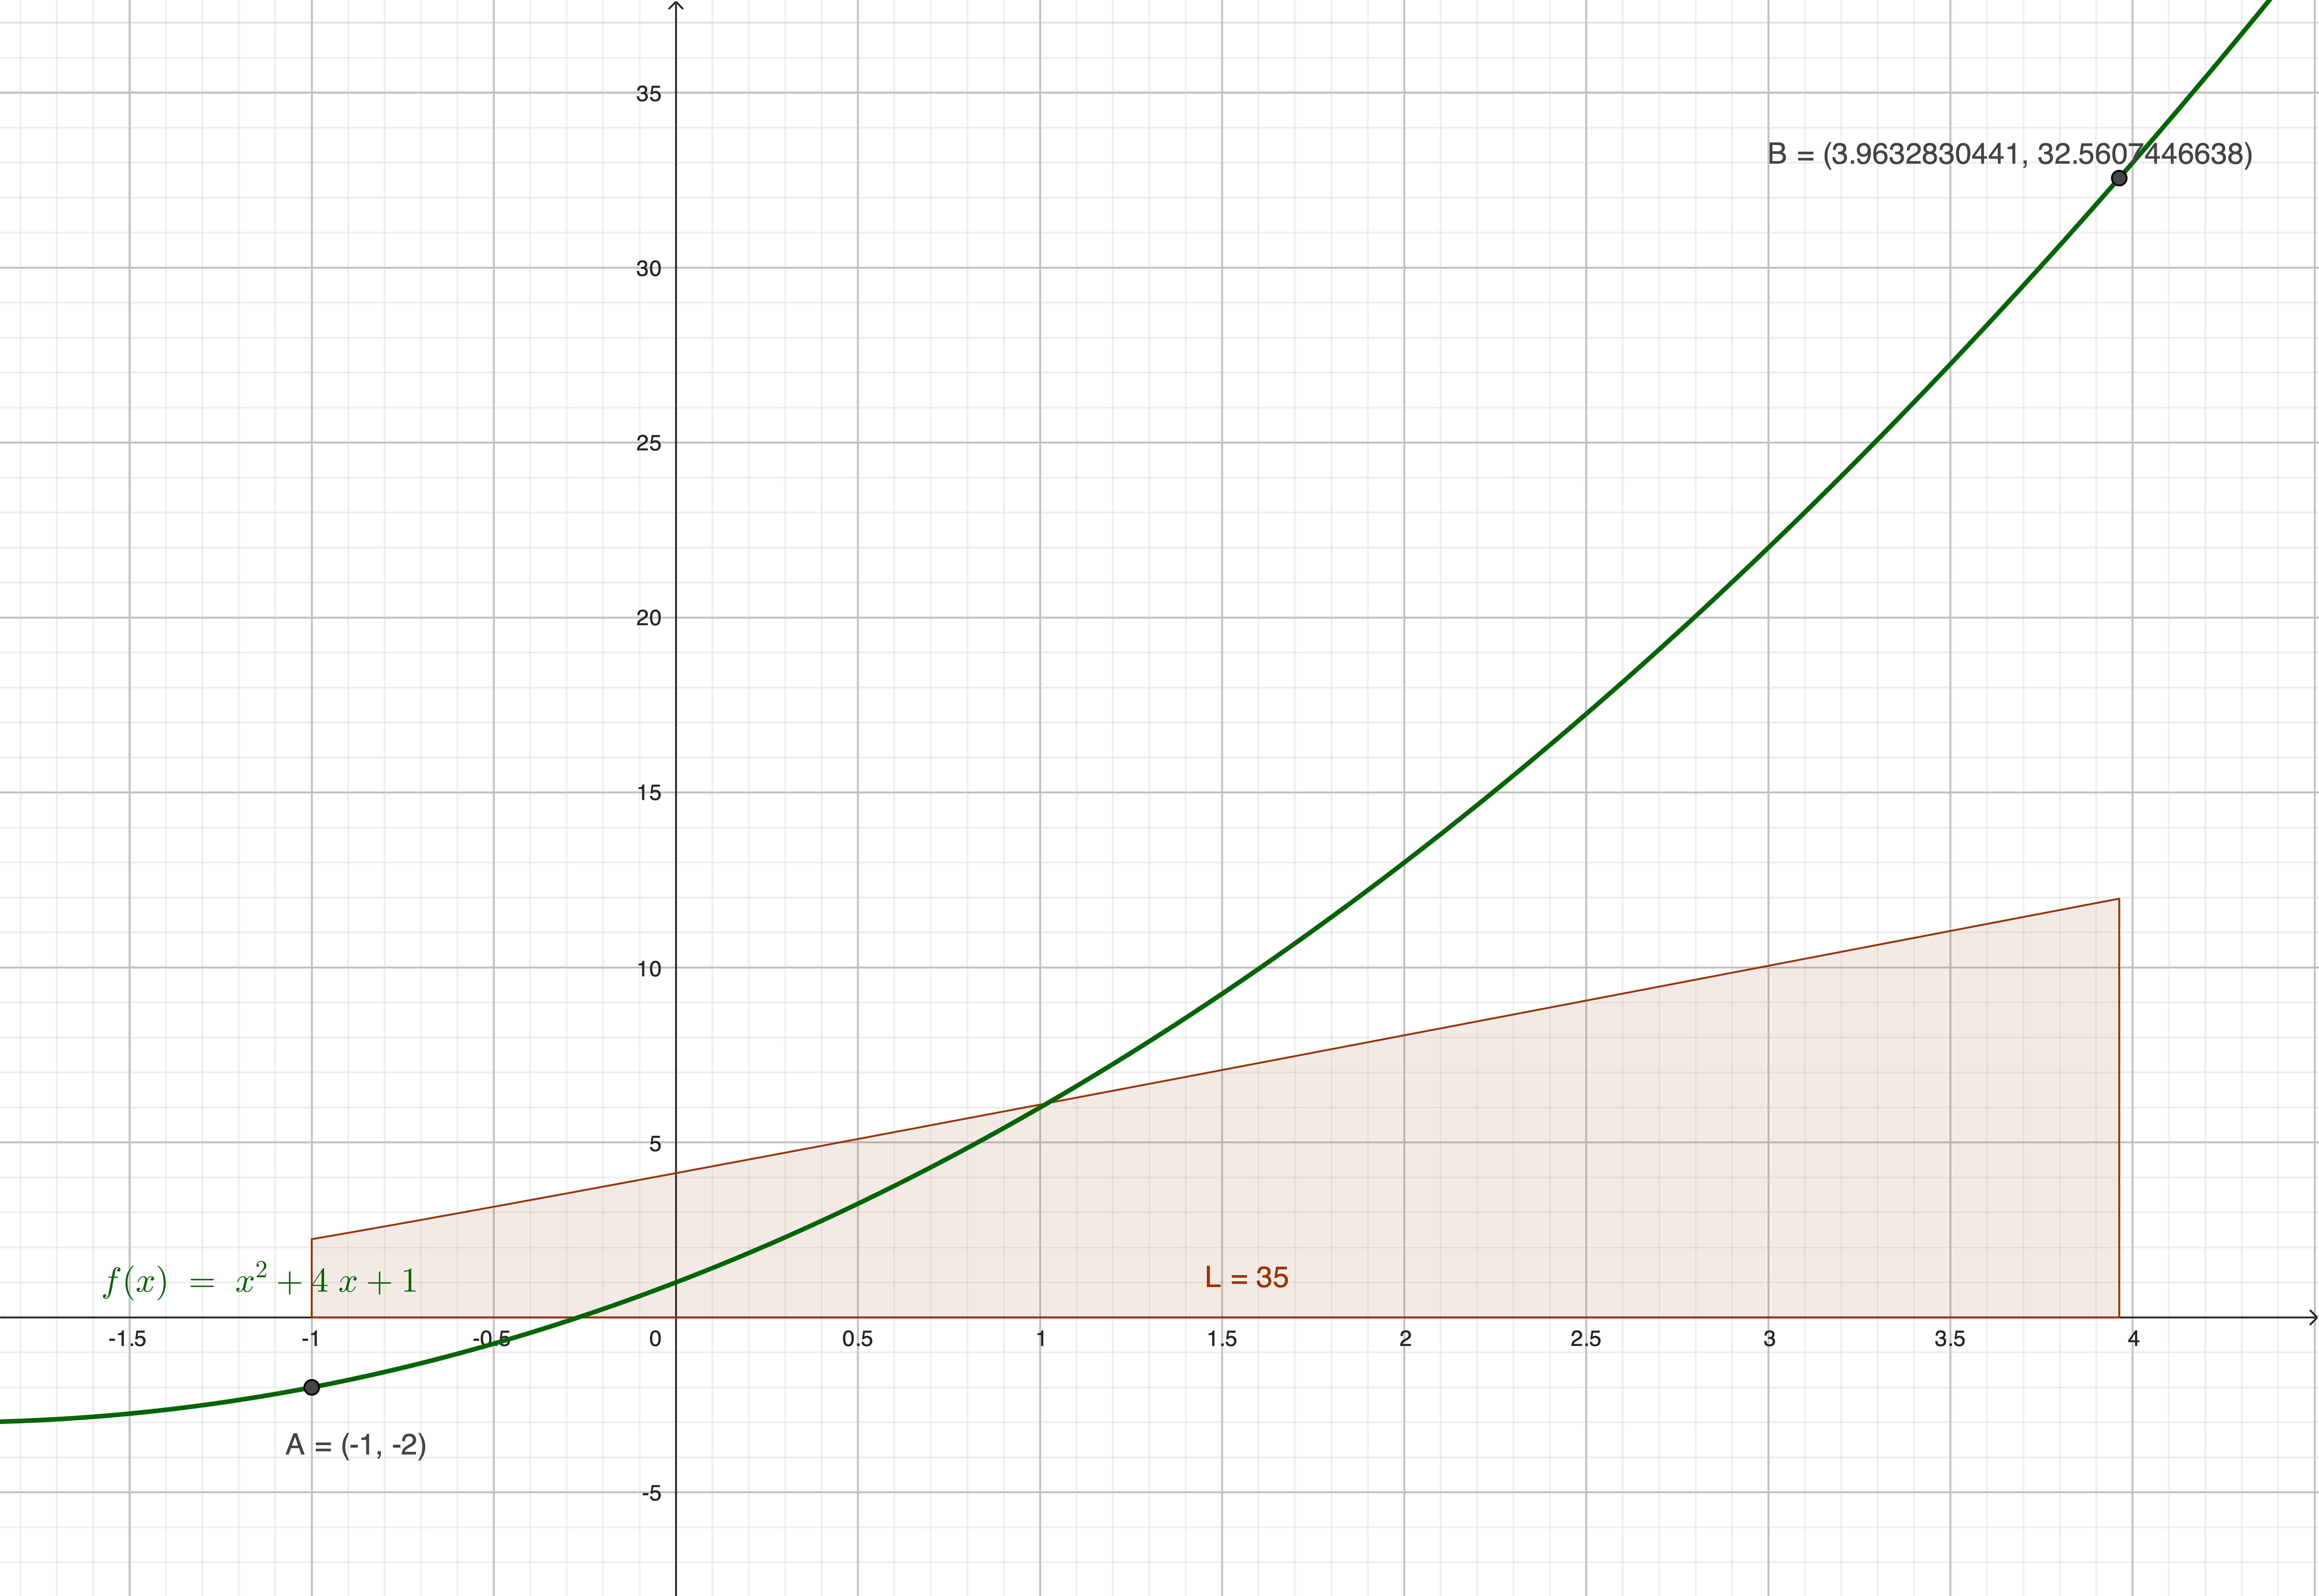
\includegraphics[scale=0.25]{graph.png}
\end{center}
\caption{Grafen for $f$, punkterne $A$ og $B$ samt den geometriske betydning af "kurvelængde-integralet" tegnet i GeoGebra}
\label{fig:graph}
\end{figure}

\begin{figure}[H]
\begin{center}
  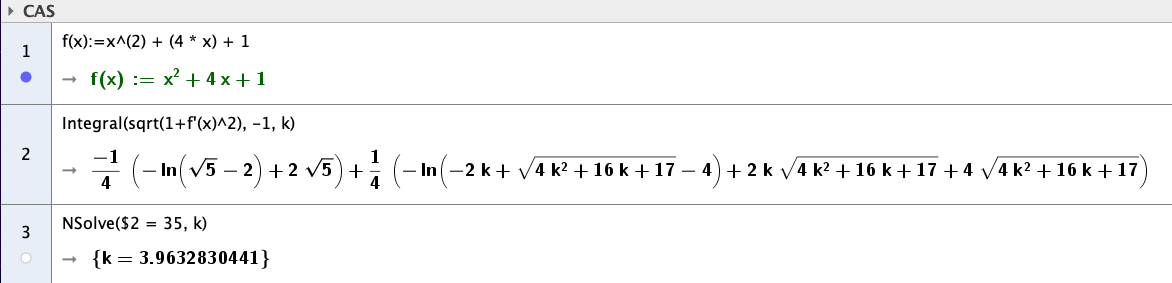
\includegraphics[scale=0.4]{CAS.png}
\end{center}
\caption{Ligningen løst numerisk med CAS}
\label{fig:CAS}
\end{figure}

\end{document}
